\documentclass[12pt]{article}

% All rights reserved.

\usepackage[ngerman]{babel} 
\usepackage[a4paper]{geometry} 
\usepackage{graphicx}
\usepackage{fancyhdr}
\usepackage{enumerate}
\usepackage{enumitem}
\usepackage{siunitx}
\usepackage[parfill]{parskip} 
\usepackage{lastpage}
\usepackage{hyperref}
\usepackage{filemod}

\geometry{
    a4paper,
    total={160mm,238mm}
}

\pagestyle{fancy}
\headheight 12mm

\renewcommand{\headrulewidth}{0.2pt} 
\renewcommand{\footrulewidth}{0.2pt}   

\setenumerate[1]{wide = 0pt,labelwidth = 1.25cm, leftmargin =!, label={\arabic*}}
\setenumerate[2]{labelwidth =1.25cm, align = left, leftmargin =0cm, label*=\Roman*}
\setenumerate[3]{labelwidth =1.25cm, align = left, leftmargin =0cm, label*=.\Roman*}

% NOTE: This line is responsible for the formatting of all our questions.
\newcommand{\question}[1]{\textit{#1}}

% Basic data
\title{\LARGE \textbf{ES-Fragestellungen}}
\date{2022/23}
\author{Die Glaubensgemeinschaft der TAEV}

\begin{document}
    \lhead{}
    \rhead{}
    \pagenumbering{Roman}

    \begin{titlepage}
        \centering
        \begin{figure}
            \centering
            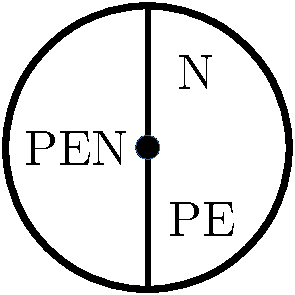
\includegraphics{nullung.pdf}
        \end{figure}

        \maketitle 
        \begin{center}
            Zuletzt aktualisiert: \textbf{\filemodprintdate{\jobname}}
        \end{center}
        \clearpage
        \tableofcontents
    \end{titlepage}

    \lhead{ES1}
    \rhead{Fragenkatalog}

    \lfoot{Zuletzt aktualisiert: \filemodprintdate{\jobname}}
    \cfoot{}
    \rfoot{Seite \thepage / \pageref{LastPage}}

    \pagenumbering{arabic}

    \section{Anlagenschutz}
    \subsection{Leitungsschutz}
Beantworten Sie folgende Fragen:

\begin{enumerate}
    \item   \question{Wodurch kann in Verteilungsnetzen (EVU-Netz, Verbraucheranlage) Überstrom auftreten?} \\\\
            Durch den Anschluss einer Überlast oder durch einen Kurzschluss.
    \item   \question{Wie erfolgt der Schutz gegen Überstrom in Verbraucheranlagen?} \\\\
            Durch Einbau von Überstrom-Schutzorganen.
    \item   \question{Welche zwei Arten von Überstromschutzorganen kennen Sie?} \\\\
            Schmelzsicherungen und Leitungsschutzschalter.
\end{enumerate}

\subsubsection{Schmelzsicherungen}
Beantworten Sie die unten aufgelisteten Aufgabestellungen. Eine Begründung Ihrer Entscheidung ist essenziell.

\begin{enumerate}
    \item   \question{Welche Bauarten werden bei Schmelzsicherungen unterschieden?} \\\\
            Es wird zwischen Stöpselsicherungen und NH-Sicherungen (Niederspannungs-Hochleistung) unterschieden.

    \item   \question{Nennen Sie die wichtigsten Kenngrößen von Schmelzsicherungen} \\\\
            Bemessungsspannung, Bemessungsstrom, Bemessungsschaltvermögen und Betriebsklasse.

    \item   \question{Über welche Prüfströme wird die Auslösecharakteristik und Fertigungstoleranz einer Schmelzsicherung festgelegt? Wie sind diese Prüfströme definiert?} \\\\
            Durch den kleinen und großen Prüfstrom. Der kleine Prüfstrom bezeichnet den Strom, bei dem die Sicherung innerhalb der konventionellen Prüfdauer nicht schmelzen darf.
            Der große Prufström beschreibt jenen Strom, bei dem die Sicherung innerhalb einer konventionellen Prüfdauer ausschalten muss.

    \clearpage
    \item   \question{Erklären Sie Aufbau und Funktion einer Stöpselsicherung (+Skizze)} \\\\
            Folgende Abbildungen zeigen den Aufbau der Stöpselsicherung.
            \begin{figure}[!htp]
                \centering
                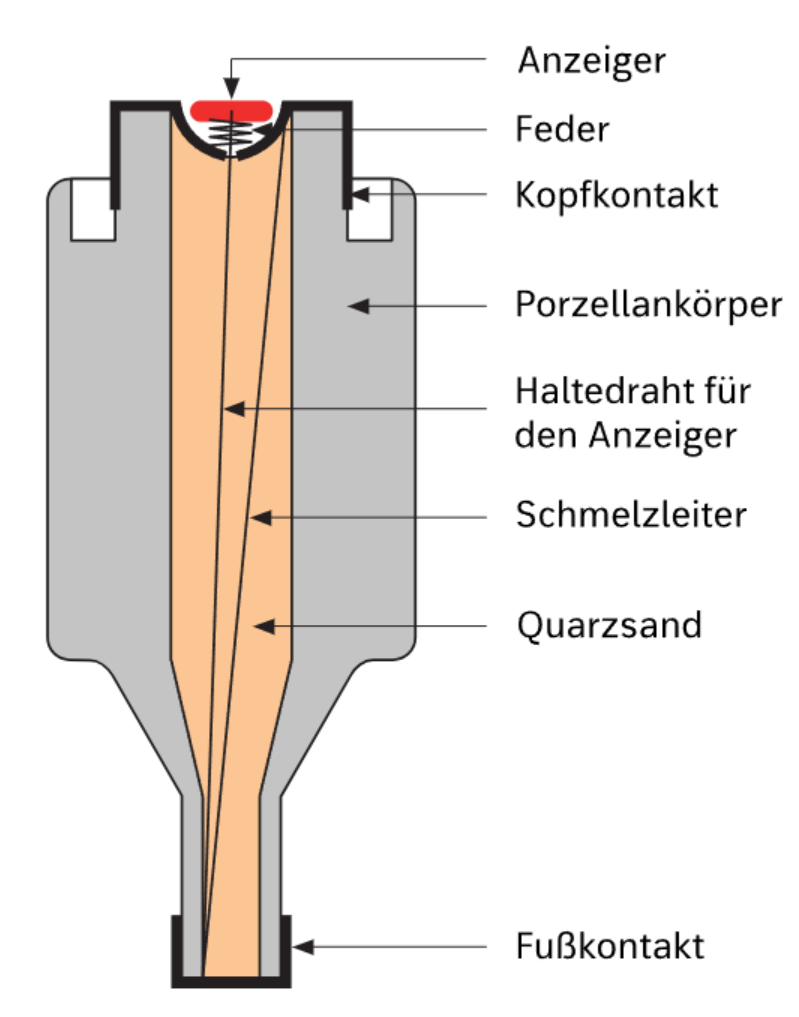
\includegraphics[scale = 0.3]{img/Stopsel_Aufbau.png}
            \end{figure}

            \begin{figure}[!htp]
                \centering
                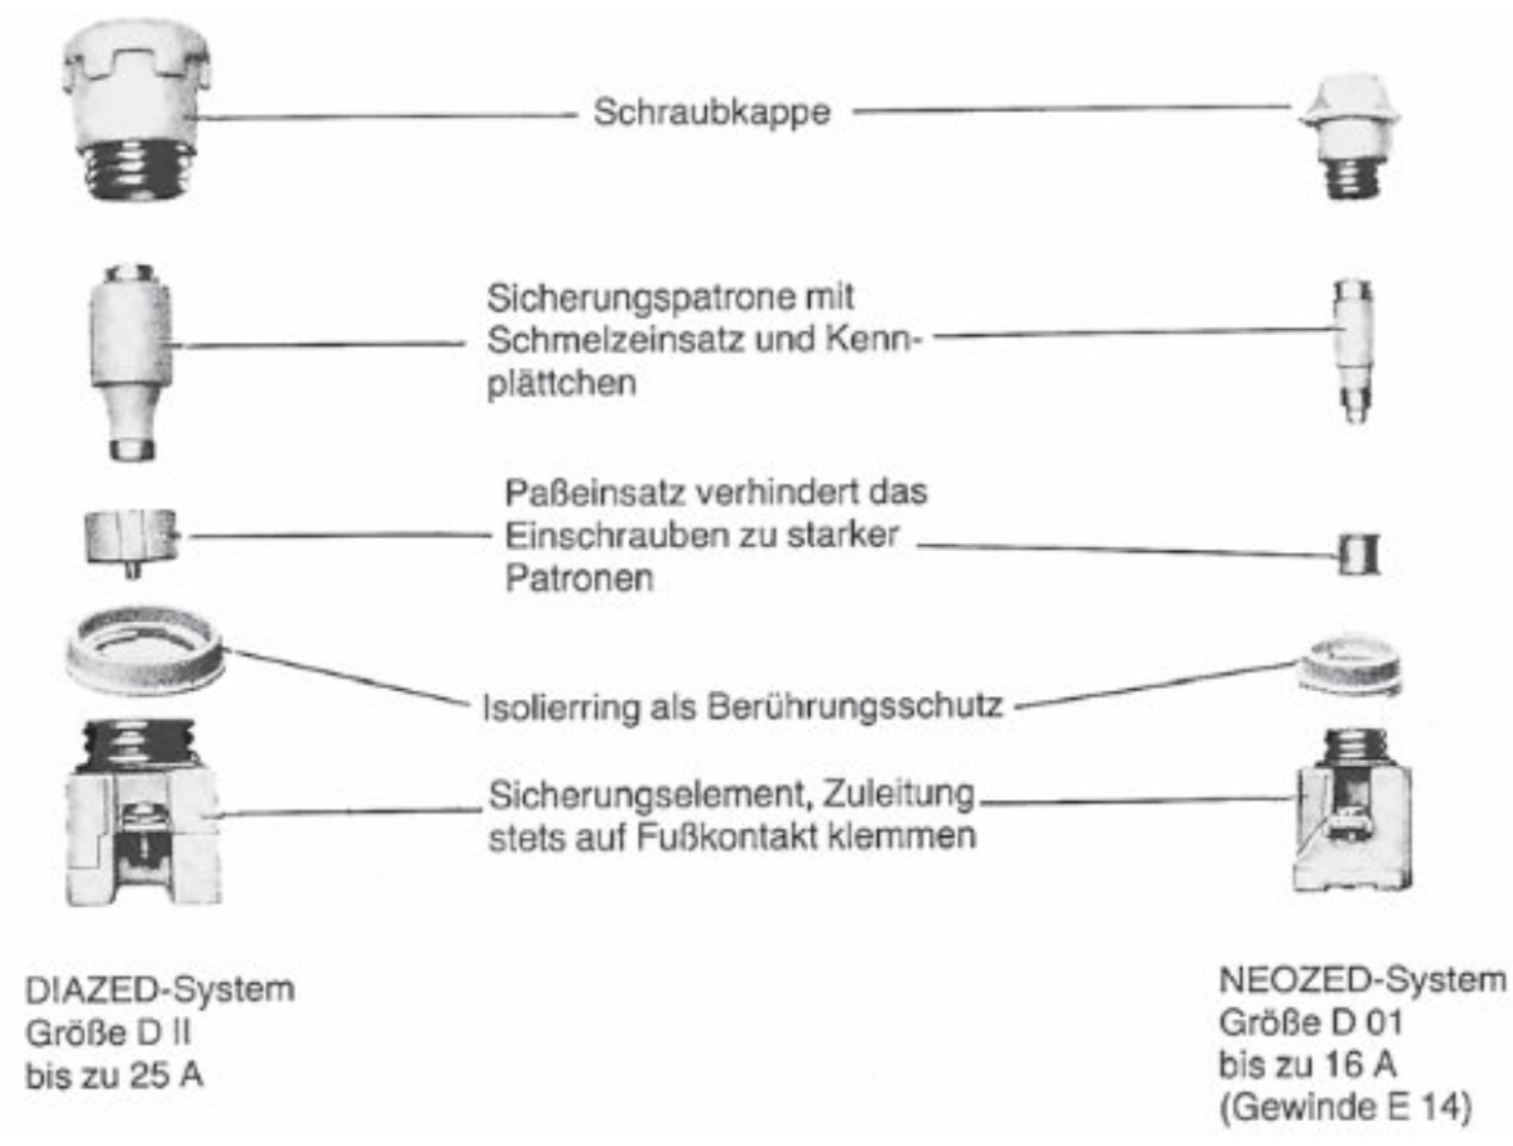
\includegraphics[width = 0.7\textwidth]{img/Stopsel_Aufbau_2.png}
            \end{figure}
            Die Sicherung stellt einen Überlastschutz und Kurzschlusschutz dar. Fließt ein zu hoher Strom, erhöht sich die Temperatur des Schmelzleiters, welcher 
            direttissima \footnote{Direttissima: Direkt; der kürzeste Weg.} schmilzt. Die Stöpselsicherungen werden heutzutage nur vereinzelt in Häusern verwendet.
            \clearpage

    \item   \question{Erklären Sie Aufbau und Funktion einer NH-Sicherung (+Skizze)}\\\\
            Folgende Abbildung zeigt den Aufbau der NH-Sicherung.
            \begin{figure}[!htp]
                \centering
                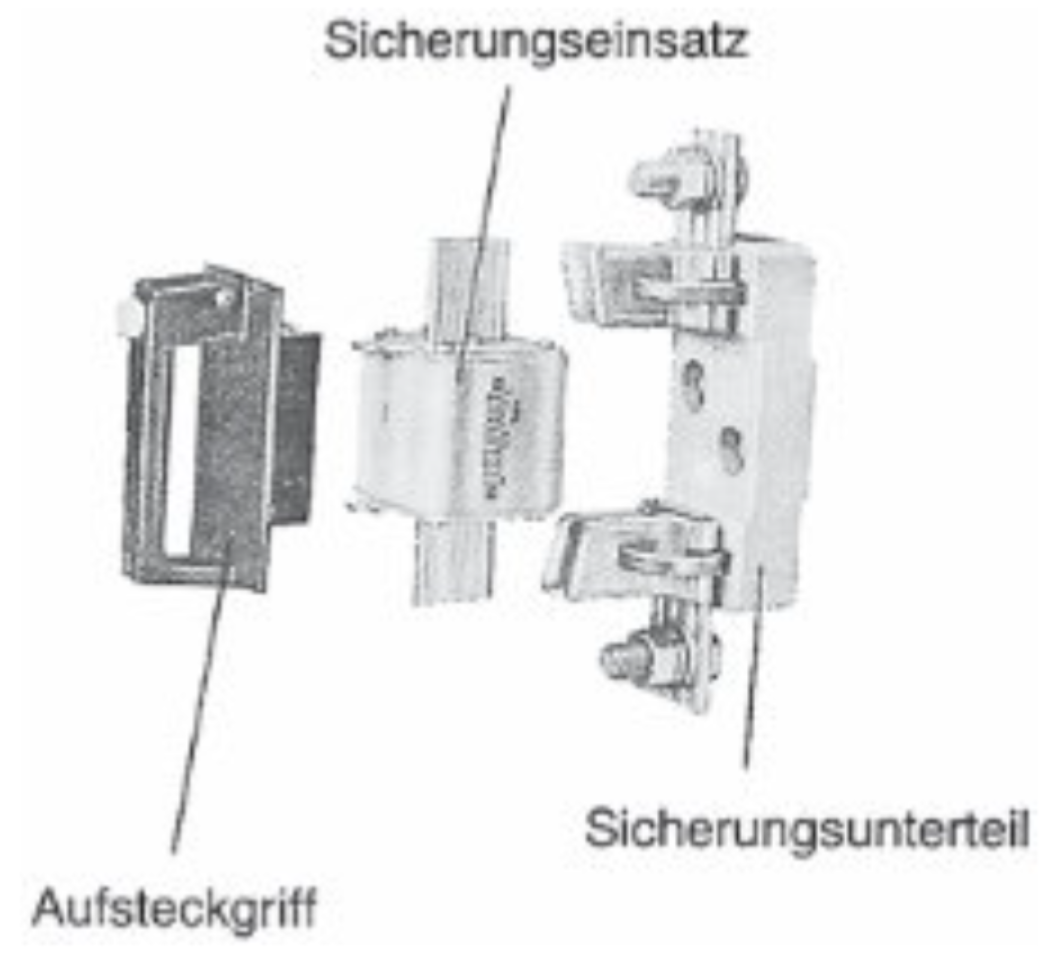
\includegraphics[scale = 0.3]{img/NH_Aufbau.png}
            \end{figure}
            \begin{figure}[!htp]
                \centering
                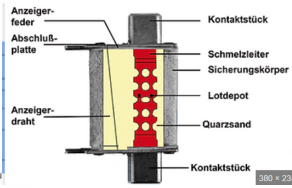
\includegraphics[scale = 0.3]{img/NH_Aufbau_real.PNG}
            \end{figure}

            Funktion: Abschaltung bei Überstrom oder Kurschluss. NH-Sicherungen sind für den Einbau in der Nähe von Transformatorstationen 
            und als Hausanschlusssicherung eingesetzt.

    \item   \question{Worüber gibt die Betriebsklasse einer Schmelzsicherung auskunft?} \\\\
            Die Betriebsklasse gibt über die Verwendbarkeit von Sicherungen und ihre Strom-Zeit-Kennlinie auskunft.

    \item   \question{Nennen Sie 3 Vorteile eines NH-Trenners gegenüber Stöpselsicherungen.} \\\\
            Ein NH-Lasttrenner bietet folgende Vorteile:
            \begin{itemize}
                \item Die massiveren Kontakte können größere Ströme führen
                \item Stromkreis wird dreipolig geschaltet
                \item Höheres Ausschaltvermögen
            \end{itemize}      

    \item   \question{Unter welchen Bedingungen werden Schmelzsicherungen gegenüber Leitungsschutzschaltern bevorzugt? (+Beispiele)}\\\\
            Wenn Selektivität benötigt wird. \textcolor{red}{Bsp.:?????}

    \clearpage


    \item   \question{Erklären Sie Aufbau und Funktion eines Leitungsschutzschalters. Wie erfolgt die Auslösung bei einem Leitungsschutzschalter.}\\\\

            \begin{figure}[!htp]
                \centering
                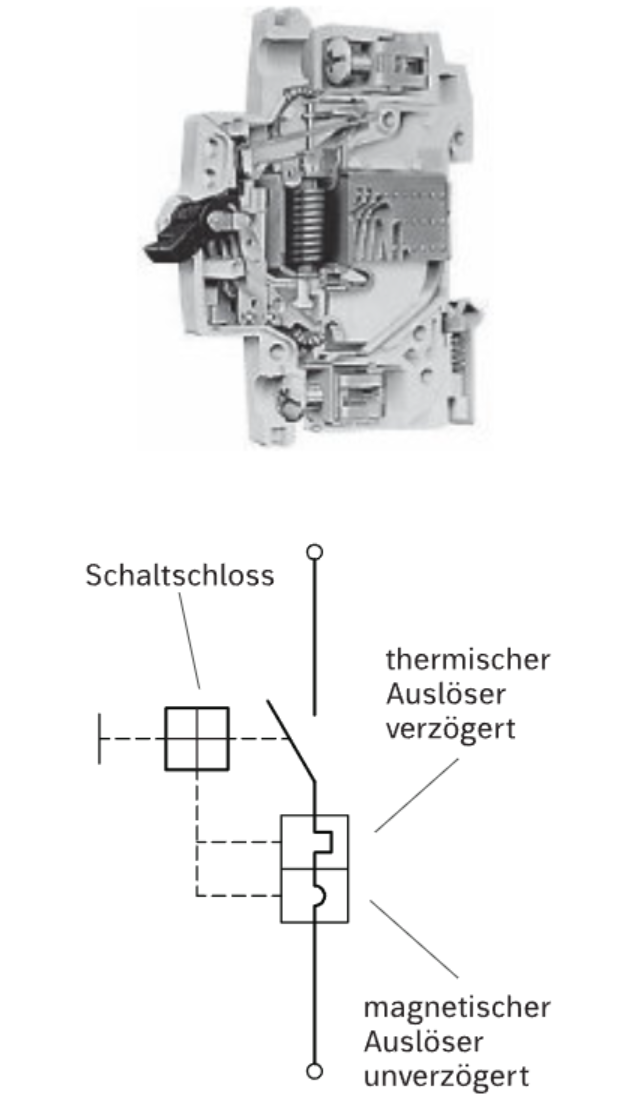
\includegraphics[width = 0.5\textwidth]{img/LSS_Aufbau.png}
            \end{figure}
            \begin{figure}[!htp]
                \centering
                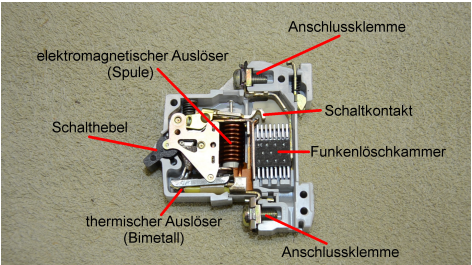
\includegraphics[width = 0.5\textwidth]{img/Leitungsschutzschalter.PNG}
            \end{figure}

            Ein Leitungsschutzschalter besitzt eine thermische (Überlastschutz) und magnetische (Kurzschlusschutz) Auslösung.

    \item   \question{Nennen Sie Vorteile von Leitungsschutzschaltern gegenüber Schmelzsicherungen.} \\\\
            Können wieder eingeschalten werden -> keine Ersatzsicherungen erforderlich -> kein Einsetzen einer falschen Sicherung möglich. Zudem lösen sie bei Kurzschlussen schneller durch. Leitungsschutzschalter lassen sich nicht überbrücken.
            Daraus folgt, dass Laien sich nicht mehr unter Gefahr setzen können. Sichere Bedienung. Kompakte Bauweise.  

    \clearpage

    \item   \question{Über welche Prüfströme  wird die Auslösecharakteristik und Fertigungstoleranz eines Leitungsschutzschalters festgelegt. Wie sind diese Prüfströme definiert?} \\\
            Es gibt folgende Auslösestrome:

            \begin{itemize}
                \item Nichtauslösestrom: jener Strom, bei dem der LSS nicht auslösen darf. 1,13-fache des Bemessungsstroms.
                \item Auslösestrom: jener Strom, bei dem der LSS innerhalb der festgelegten Prüfdauer ausschalten \textbf{muss}. 1,45-fache des Bemessungsstroms.
                \item Sofortauslösestrom: jener Strom, bei dem der LSS innerhalb $\SI{0.1}{s}$ abschaltet. Er hängt von der Type ab.
            \end{itemize}

    \item   \question{Wie unterscheiden sich Leitungsschutzschalter der Typen B, C und D in ihrer Auslösecharakteristik (+Skizze)?} \\\\
            Folgende Skizze beschreibt den Unterschied:

            \begin{figure}[!htp]
                \centering
                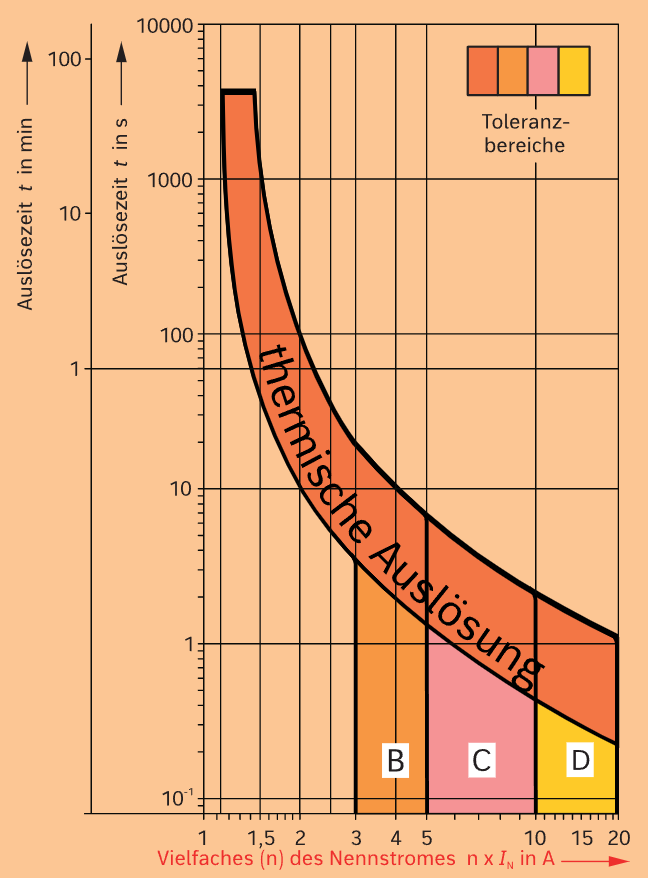
\includegraphics[width = 0.5\textwidth]{img/Auslosecharakteristik.png}
            \end{figure}

            Die thermische Auslösung ist äquivalent. Sie unterscheiden sich nur durch die magnetische Auslösung.
            Desto höher der Buchstabe, desto niedriger die Sensitivität über Spitzenströme.

    \clearpage

    \item   \question{Ein Winkelschleifer hat einen Nennstrom von 6A und nimmt beim Einschalten kurzzeitig den 8fachen Strom auf. Wird ein klagloser Betrieb möglich sein, wenn der Stromkreis mit einem 13A LS-Schalter vom Typ B abgesichert ist oder schlagen Sie einen anderen Leitungsschutzschalter vor? (+Begründung)} \\\\
            \textcolor{red}{TODO.} Ein Typ-C-Leitungsschutzschalter ist empfehlenswert.

    \item   \question{Worauf muss man bei der Verwendung von LS-Schaltern der Type D im genullten Netz achten?} \\\\
            Die Ausschaltbedingung muss erfüllt sein. Ist diese nicht erfüllt, so ist die Nullung nicht wirksam. Es besteht Lebensgefahr.

            Anhand folgender Formel lässt sich dies erklären:

            $$Z_S \le \frac{U_0}{I_A}$$

            $I_A$ ist bei Type D besonders groß. 

    \item   \question{Was versteht man unter der Energiebegrenzungsklasse eines Leitungsschutzschalters? Welche Auswirkung hat eine hohe Energiebegrenzungsklasse?} \\\\
            Die Energiebegrenzungsklasse eines LS-Schalters ist ein Maß für die Durchlassenergie, die ein Schalter benötigt, um den Stromkreis zu öffnen $\left(I^2\cdot t\right)$.
            Es gibt die Energiebegrenzungsklassen 1, 2 und 3. Je höher, desto niedriger ist die spezifische Durchlassenergie (bezogen auf den Bemessungsstrom), desto schneller schaltet der Schalter aus.         
\end{enumerate}

\subsubsection{Ausschaltstrom / Selektivität}
Lösen Sie folgende Aufgabenstellungen zum Thema Ausschaltstrom / Selektivität

\begin{enumerate}
    \item   \question{Wie ist der Ausschaltstrom von Überstromschutzorganen definiert?} \\\\
            Der Ausschaltstrom ist jener Strom, der fließen muss, damit ein Überstromschutzorgan im Fehlerfall so schnell ausschaltet, dass keine Gefahr durch indirektes Berühren entsteht.
            Dieser Strom wird als Vielfache des Nennstromes angegeben.

    \item   \question{Was versteht man unter Selektivität von Überstromschutzorgangen? Unter welcher Voraussetzung ist die Selektivität gegeben? Nennen Sie 2 einfache Regeln zur Selektivität.} \\\\
            Selektivität bedeutet, dass im Fehelrfallse nur jenes Überstromschutzorgan abschaltet, das sich unmittelbar vor der Fehlerstelle befindet, und alle anderen betriebsbereit bleiben.
            Durch die Selektivität wird die Betriebssicherheit einer Anlage erheblich verbessert.
            2 Regeln: \\
            - Schmelzsicherungen sind bei einem Nennstromverhältnis von 1 : 1,6 selektiv. \\
            - In der Reihe geschaltete Leitungsschutzschalter sind in der Regel bei Kurzschluss nicht selektiv (beide magnetischen Auslöser schalten ab).  
\end{enumerate}
    \subsection{Bemessungskriterien}
\subsubsection{Anordnung von Leitungsschutzorganen}

Lösen Sie folgende Aufgabenstellungen:
\begin{enumerate}
    \item   \question{An welcher Stelle einer Leitung sind Überstromschutzorgane anzubringen?} \\\\
            An allen Stellen, an denen eine Änderung des 
            \begin{itemize}
                \item Querschnitts
                \item Verlegungsart
                \item Leitungsaufbaus
            \end{itemize}

            den zulässigen Dauerstrom $I_Z$ reduziert.
    \item   \question{Darf der N-Leiter mit einem eigenen Überstromschutzorgan abgesichert werden? \\ a) Wird empfohlen \\ b) Ja \\ c) Nein \\[\baselineskip] (Antwort + Begründung + Bedingungen)} \\\\
            Nein! Löst der LSS aus, so würde sich trotz eines ausgelösten LSS eine Spannung in Geräten befinden. Dies kann eine Gefahr bei der Fehlersuche darstellen.
    \item   \question{Darf der N-Leiter gemeinsam mit dem Überstromschutzorgan der Aussenleiter abgesschaltet werden? \\ a) Wird empfohlen \\ b) Ja \\ c) Nein \\[\baselineskip] (Antwort + Begründung + Bedingungen)} \\\\
            TODO
    \item   \question{Darf der PE-Leiter mit einem eigenen Überstromschutzorgan abgesichert werden? \\ a) Wird empfohlen \\ b) Ja \\ c) Nein \\[\baselineskip] (Antwort + Begründung + Bedingungen)} \\\\
            Nein, behinderung der Schutzmaßnahmen mit Schutzleiter.
    \item   \question{Darf der PE-Leiter gemeinsam mit dem Überstromschutzorgan der Aussenleiter abgesschaltet werden? \\ a) Wird empfohlen \\ b) Ja \\ c) Nein \\[\baselineskip] (Antwort + Begründung + Bedingungen)} \\\\
            Nein, behinderung der Schutzmaßnahmen mit Schutzleiter.
    \item   \question{Darf der Überstromschutz vom Kurzschlussschutz getrennt werden? (+Beispiel) An welcher Stelle der Leitung können die jeweiligen Schutzorgane angebracht werden?} \\\\
            Ja, beispielsweise bei Motoren. Thermorelais + Schmelzsicherungen. Der Kurzschlusschutz muss grundsätzlich an dem Leitungsanfang platziert werden.
            (Er lässt sich unter bestimmten Bedingungen verschieben) Der Überstromschutz kann beliebig verschoben werden.
\end{enumerate}

\subsubsection{Schaltanlage / graphische Symbole}
Lösen Sie die unten aufgelisteten Aufgabenstellungen.

\begin{enumerate}
    \item   \question{Zeichnen Sie das Symbol einer Schmelzsicherung für Drehstromanschluss (einpolige und mehrpolige Darstellung)}
    \item   \question{Zeichnen Sie das Symbol eines Leitungsschutzschalters für Drehstromanschluss (einpolige und mehrpolige Darstellung)}
\end{enumerate}

    \section{Lichttechnik}
    \subsection{Licht und Wahrnehmung}
Beantworten Sie folgende Fragen zum Thema Licht und Wahrnehmung.
\begin{enumerate}
    \item   \question{In welchem Wellenlängenbereich der elektromagnetischen Strahlung kann das menschliche Auge Licht wahrnehmen?}\\\\
            Der Bereich liegt zwischen $\SI{380}{nm}-\SI{780}{nm}$.

    \item   \question{Bei welcher Wellenlänge liegt die größte Hellempfindlichkeit für\\ a) Tagsehen \\b) Nachtsehen}\\\\
            $\SI{550}{nm}$ und $\SI{505}{nm}$ respektive.

    \item   \question{Was versteht man unter Akkomodation des Auges?}\\\\
            Die Akkomodation ermöglicht eine Veränderung der Brennweite. Somit kann das Auge auf ein
            näheres Objekt fokussieren.

    \item   \question{Was versteht man unter Adaption des Auges und welche Abläufe im Auge ermöglichen die Adaption?}\\\\
            Anpassung an Lichtvehältnissen. Die Iris wirkt wie eine Blende bei handelsüblichen Kameraapparaten. Sie kann sich für helle Szenen 
            zusammenziehen und bei dunklen Szenen weiten.
    \clearpage
    \item   \question{Wie entstehen die Farben aus den Grundfarben über additive Farbmischung?}\\\\
            Ausgehend von Schwarz wird die Ergebnisfarbe heller, je mehr Grundfarbe hinzugegeben wird.
    \item   \question{Wie entstehen die Farben aus den Grundfarben über subtraktive Farbmischung?}\\\\
            Ausgehend von einem definierten Frequenzspektrum wird die Ergebnisfarbe dunkler, je mehr Frequenzanteile herausgefilter bzw. absorbiert werden.

    \item   \question{Was versteht man in der Lichttechnik unter einem kontinuierlichen Spektrum. Nennen Sie Beispiele für Lichtquellen mit kontinuierlichem Spektrum.} \\\\
            Tageslicht hat eine durchgängige spektrale Strahlungsverteilung: Ein kontinuierliches Spektrum. Nur Temperaturstrahler (Glühlampen, Halogenlampen) weisen ein kontuierliches Spektrum auf.

    \item   \question{Was versteht man in der Lichttechnik unter einem diskreten Spektrum? Nennen Sie Beispiele für Lichtquellen mit diskretem Spektrum.}\\\\
            Ein diskretes Spektrum weist eine unterschiedliche spektrale Verteilung auf. Beispiele sind Entladungslampen.

    \item   \question{Was versteht man unter Farbtemperatur: Wie ist sie definiert und in welcher Einheit wird sie angegeben?}\\\\
            Sie ist ein Maß, um den Farbeindruck einer Lichtquelle zu beschreiben. Die Einheit der Farbtemperatur ist Kelvin. Darunter versteht man ebenfalls jene Glühtemperatur, auf die man den „schwarzen Körper“ bringen müsste, damit er Licht gleicher Farbe aussendet wie die zu untersuchende Lichtquelle.


    \item   \question{Was versteht man unter dem Farbwiedergabeindex (CRI) $R_a$? Wie wird der Farbwiedergabeindex berechnet?}\\\\
            Der Farbwiedergabeindex gibt an, wie farbecht Farben unter künstlichem Licht dargestellt werden.
            Der CRI wird berechnet, indem die Farben von acht Standardfarben unter der zu testenden Lichtquelle mit den Farben unter einer Referenzlichtquelle verglichen werden.

    \item   \question{Was bedeutet eine Kennzeichnung mit den drei Ziffern 950 auf dem Sockel eines Leuchtmittels?}\\\\
            Das Leuchtmittel weist eine Farbwiedergabestufe von A1 (90\%) sowie eine Farbtemperatur von $\SI{5}{kK}$ auf. Es wird als 
            Neutralweiß bezeichnet.
\end{enumerate}

\clearpage

\subsubsection{Lichttechnische Größen}
Arbeiten Sie folgende Aufgabenstellung genau und zielführend durch:

\begin{enumerate}
    \item   \question{Nennen sie die vier lichttechnischen Grundgrößen und ihre Einheiten sowie die Bedeutung dieser Größen.} \\\\
            
            Es wird zwischen folgenden Größen unterschieden:
            \begin{itemize}
                \item \textbf{Lichtstrom $\phi$}: $\left[\phi\right] = \textnormal{lm}$ \\ Die gesamte von einer Lichtquelle abgegebene und vom Auge bewertete Strahlungsleistung. Durch Lampenhersteller angegeben.
                \item \textbf{Lichtstärke $I$}: $\left[I\right] = \textnormal{cd}$ \\ Sie ist ein Maß für die Intensität des Lichts in einer bestimmten Richtung.
                \item \textbf{Beleuchtungsstärke $E$}: $\left[E\right] = \textnormal{lx}$ \\ Sie ist das Verhältnis von Lichtstrom zur Fläche, auf die der Lichtstrom auftritt
                \item \textbf{Leuchtdichte $L$}: $\left[L\right] = \frac{cd}{m^2}$
            \end{itemize}

    \item   \question{Wie heißt die lichttechnische Größe und Einheit, mit der die gesamte, von einer Lichtquelle abgegebene und vom Auge bewertete Strahlungsleistung gemessen wird?} \\\\
            Die Größe ist der Lichtstorm $\phi$. Es gilt: $\left[\phi\right] = \textnormal{lm}$

    \item   \question{Wie errechnet sich die Lichtausbeute einer Lichtquelle (Formel angeben)?}
            $$\textnormal{Lichtausbeute} = \frac{\phi}{P}$$

    \item   \question{Auf welche lichttechnische Größe bezieht sich die Energieeffizienzklasse, die entsprechend der EU-Richtlinie auf der Verpackung von Leuchtmitteln angegeben ist?} \\\\
            Die Energieeffizienzklasse bezieht sich auf die Lichtausbeute.

    \item   \question{Wie heißt die lichttechnische Größe und Einheit, mit der die gesamte, auf einer Fläche auftreffende und vom Auge bewertete Strahlungsleistung $\phi$ im Verhältnis zur Flächengröße gemessen $A$ wird?}\\\\
            Beleuchtungsstärke.
    \item   \question{Wie errechnet sich die Beleuchtungsstärke aus $\phi$ (Formel angeben)?}
            $$E = \frac{\phi}{A}$$
    \item   \question{Wie errechnet sich die horizontale Beleuchtungsstärke aus $I$?}
            $$E_H= \frac{\vec{I}}{h^2} \cdot \cos^3\left(\alpha\right)$$ \Huge Eventuell wird eine Frage gestellt. \normalsize
    \item   \question{Wie errechnet sich die vertikale Beleuchtungsstärke aus $I$?}
            $$E_V = \frac{\vec{I}}{r^2} \cdot \sin \left(\alpha\right)$$
    \item   \question{Was ist eine Lichtverteilungskurve? Erklären Sie anhand der C-Ebene den Zusammenhang zwischen Lichtverteilungskurve und Lichtverteilungskörper.}\\\\
            Mit den Lichtstärkeverteilungskurven einer Lampe oder Leuchte kann man die Lichtstärke für
            beliebige Raumwinkel darstellen.
            
    \item   \question{Erklären Sie den Zusammenhang zwischen Lichtstrom und Lichtstärke.}
            $$I_V = \frac{\textnormal{d}\Phi_V}{\textnormal{d}\Omega}$$

            $\Phi$ ... gesamter Lichtstrom der Lichtquelle\\
            $\textnormal{d}\Omega$ ... differentieller Raumwinkel\\
            $\Phi_V$ ... Lichtstrom der Lichtquelle in Richtung des differentiellen Raumwinkels

    \item   \question{Wie groß ist die Beleuchtungsstärke, wenn ein Lichtstrom $\Phi = \SI{800}{lm}$ gleichmäßig und normal auf eine Fläche von $A = \SI{6}{m^2}$ auftrifft?}
            $$E = \frac{\Phi}{A} = \frac{\SI{800}{lm}}{\SI{6}{m^2}} = \SI{133.3}{lx}$$
\end{enumerate}


    \subsection{Leuchtmittel}
\subsubsection{Prinzipien}
Arbeiten Sie folgende Aufgabenstellung durch:

\question{Nach welchen Prinzipien funktioniert die Umwandlung elektrischer Energie in Licht?}
Fragen: Lumineszenz / LED.

\subsubsection{Beleuchtungskörper}

Arbeiten Sie die unten aufgelistete Aufgabenstellung durch.

\clearpage

\begin{enumerate}
    \item   \question{Skizzieren und erklären Sie die induktive Schaltung einer Leuchtstofflampe mit konventionellem Vorschaltgerät}\\
            
            Fragen: Welches Detail wird bei der Erklärung benötigt.

            \begin{figure}[!htp]
                \centering
                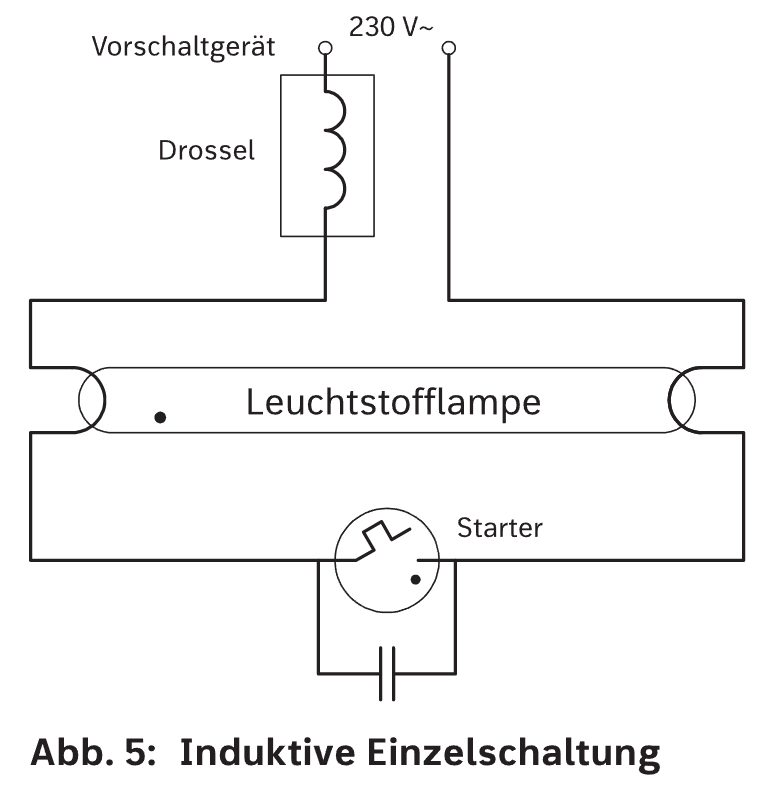
\includegraphics[scale = 0.3]{img/induktive_einzelschaltung.png}
            \end{figure}

    \item   \question{Skizzieren und erklären Sie die kapazitive Schaltung einer Leuchtstofflampe mit konventionellem Vorschaltgerät. Wo wird diese Schaltung eingesetzt, welche Vorteile hat sie?}\\
            
            Fragen: Welches Detail wird bei der Erklärung benötigt.

            \begin{figure}[!htp]
                \centering
                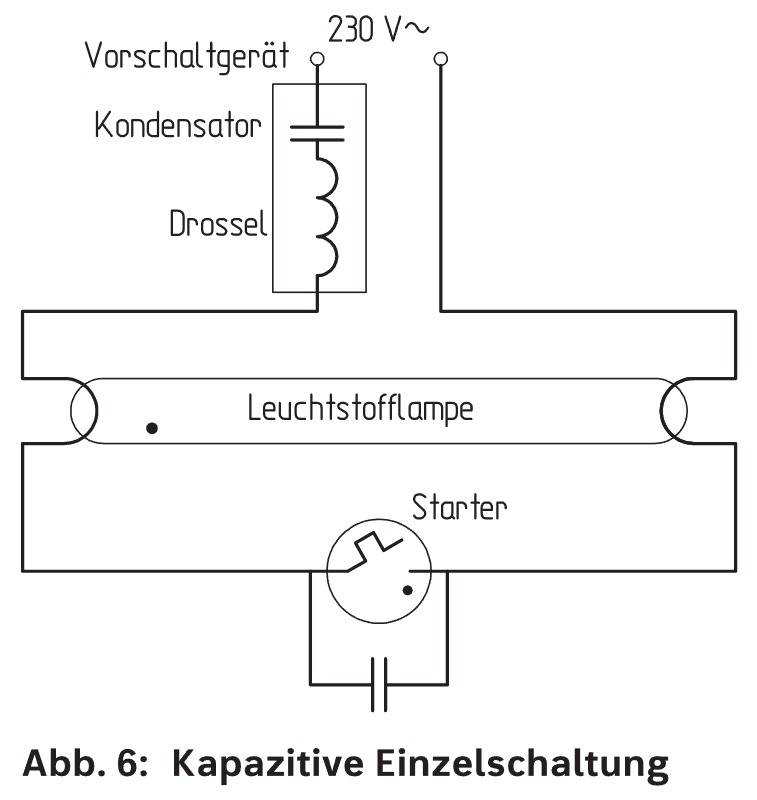
\includegraphics[scale = 0.3]{img/kapazitive_einzelschaltung.png}
            \end{figure}

            \clearpage
    
    \item   \question{Skizzieren und erklären Sie die Duo-Schaltung bei Leuchtstofflampen mit konventionellen Vorschaltgeräten. Wo wird diese Schaltung eingesetzt, welche Vorteile hat sie?}\\
            
            Fragen: Welches Detail wird bei der Erklärung benötigt.

            \begin{figure}[!htp]
                \centering
                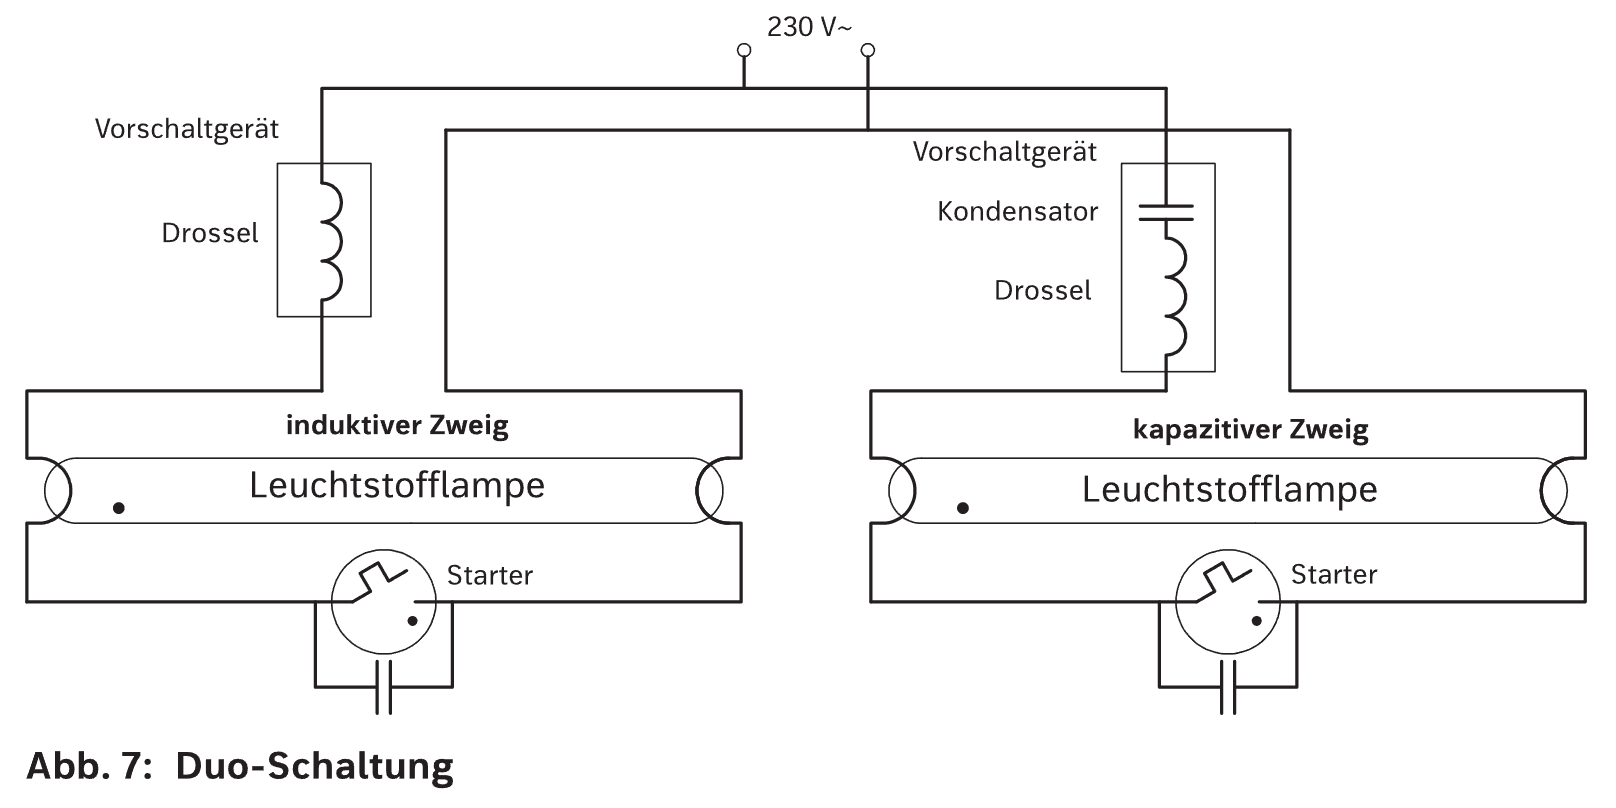
\includegraphics[scale = 0.3]{img/duo_schaltung.png}
            \end{figure}

    \item   \question{Wie wird bei Leuchtstofflampen der Zündvorgang hervorgerufen? Welche Vorschaltgeräte werden unterschieden und welche Vor- und Nachteile haben diese Vorschaltgeräte?}\\
    
    Mit Hilfe des Startes wird der Zündvorgang eingeleitet. Prinzip von einem Starter:
    \\1.    Lampe einschalten: Volle Spannung am Starter - Bildung einer Glimmentladung in der Edelgasatmosphäre - Erwärmung der Bimetallstreifen
    \\2.    Kurzschließen der Glimmstrecke durch die starke Biegung der Bimetallstreifen - Aufheizung der Lampenelektroden
    \\3.    Glimmentladung stoppt, Bimetallstreifen kühlt ab und öffnet - Unterbrechen von Heizkreis
    \\4.    An der Drosselspule tritt eine Selbstinduktionsspannung auf und dadurch erfolgt die Zündung

    \item   \question{Nach welchem Prinzip funktioniert eine Leuchtstofflampe?}\\
    
            Fragen: Detail der Antwort ausreichend?        

            Gasentladungsprinzip

            \clearpage
            
    \item   \question{Welche Gasentladungslampen kennen Sie und wo werden diese angewendet?}\\
    
            \begin{itemize}
                \item Natriumdampfhochdrucklampen\\
                    Beleuchtung von Straßen u. Plätzen. \\
                    In Neuanlagen werden statt Niederdrucklampen fast ausschließlich Hochdrucklampen verwendet.

                \item Natriumdampfniederdrucklampen\\
                    Ausfallsstraßen, Hafenanlagen, Schiffswerfen, Lagerhallen, u.ä.\\
                    Werden verwendet wenn Preis im Vordergrund steht. Keine Farbwiedergabeeigenschaften werden benötigt.

                \item Xenonlampen\\
                    Nach Beispielen Fragen. Laut Wikipedia:\\
                    Fahrzeugscheinwerfer, Großkinofilmprojektoren, Leuchtürme, für Wissenschaftliche Anwendungen
            \end{itemize}

    \item   \question{Lichttechnik: Welche thermischen Strahler kennen Sie und welche Vor- und Nachteile haben diese?}\\
            
            \begin{itemize}
                \item Glühlampe\\
                    Vorteile: Kontinuierliches Spektrum, hohe Farbtreue, (warm :3)
                    Nachteile: Schlechter Wirkungsgrad (Große Wärmeverluste)

                \item Halogenlampen (Vor- u. Nachteile siehe unten)
            \end{itemize}


    \item   \question{Nach welchem Prinzip funktioniert eine Halogenleuchte? Welche Vor- und Nachteile bietet eine Halogenleuchte gegenüber anderen Leuchtmitteln?}\\
    
    Um das abschlagen von Wolfram am Glaskolben zu verhindern, wird bei dieser Lampe Jod eingebracht. In Lampenkolbennähe bildet
    sich Wolframjodid, das in Wendelnähe durch die hohe Temperatur wieder in Wolfram und
    Jod zerfällt.
    
    Da Glaskolben und Wendel verschiedene Temperaturen besitzen, kommt es zu einem
    Kreisprozess, und das vom Leuchtkörper abgetragene Wolfram wird nach vorübergehender
    Bindung an Jod wieder in Wendelnähe zurückgebracht.
    
    Niederschlagen von Wolfram am Kolben wird verhindert.
    
    Wegen der höheren Temperatur wird Quarzglas verwendet.
    
    Halogenglühlampen haben die gleichen Betriebseigenschaften wie gasgefüllte Glühlampen.

            Fragen: Mehr Nachteile?\\
            Vorteile: Kleine Abmessungen, hohe Lebensdauer, hohe Lichtausbeutung (bis zu $27\frac{\textnormal{lm}}{\textnormal{W}}$), kein Lichtstromabfall durch Kolbenschwärzung\\
            Nachteile: Schlechter Wirkungsgrad
\end{enumerate}
\end{document}